\section{Aktør diagram}
%Følgende afsnit beskriver aktørerne i systemet.
Nedenstående figur viser hvilke aktører der interagerer med systemet.

\begin{figure}[H]
\centering
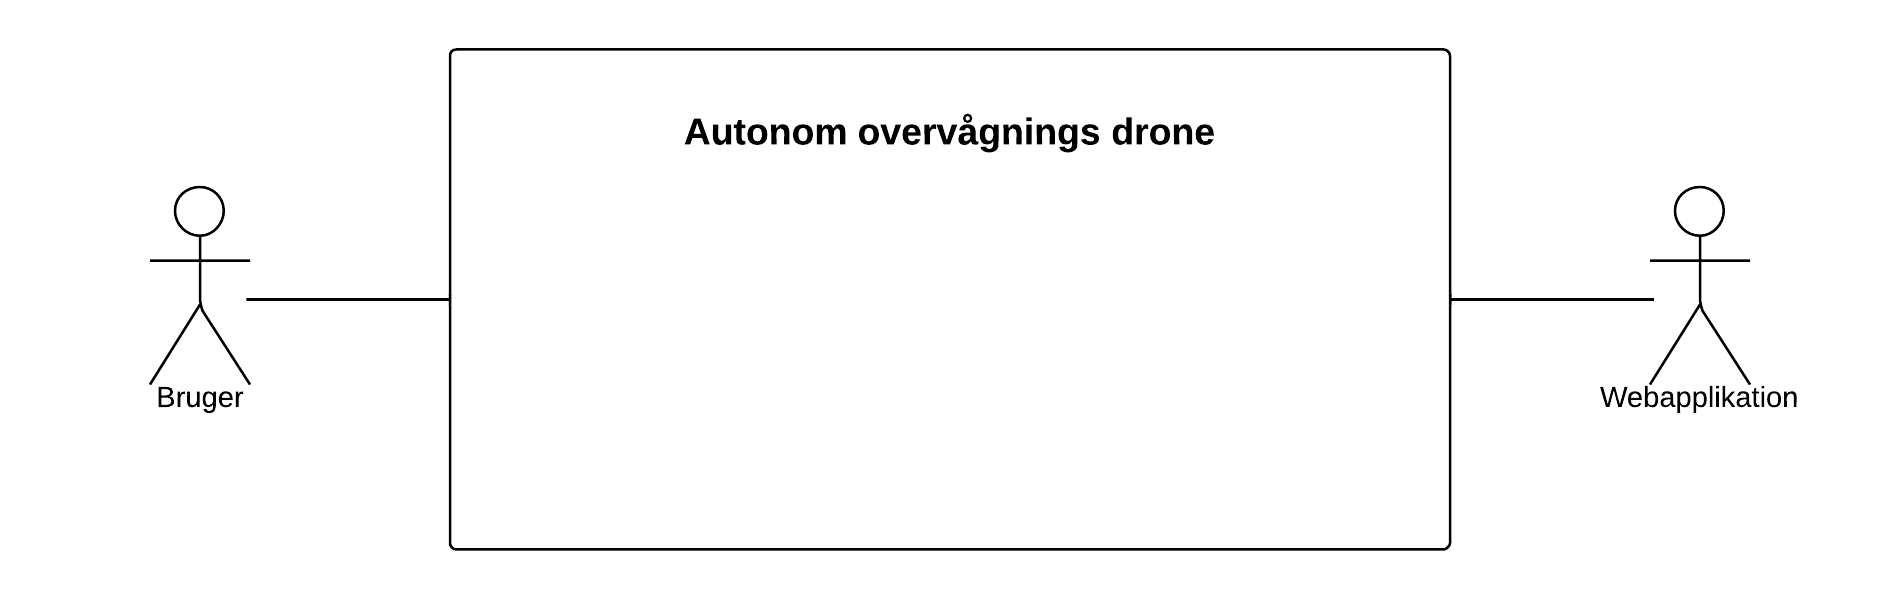
\includegraphics[width=1\textwidth]{Billeder/Aktor_diagram.png}
\caption{Aktør diagram}
\label{fig:ATD}
\end{figure}

\section{Aktørbeskrivelser}
Aktørbeskrivelsen skitserer systemets aktører samt hvilken rolle de spiller for systemet.


\begin{table}[H]
\begin{tabular}{|l|p{12.25cm}|} \hline

Navn					& Bruger. 	\\\hline
Type					& Primær.	\\\hline
Beskrivelse				& Bruger er den eneste person der interagerer med systemet.\\
						& Via webapplikation indstiller bruger flyveopsætning for nye flyvninger, samt undersøge billeder og flyveruter fra tidligere flyvninger.\\\hline
						
\end{tabular}
\caption{Aktørbeskrivelse, Bruger}
\label{tab:AB1}
\end{table}


\begin{table}[H]
\begin{tabular}{|l|p{12.25cm}|}
\hline
Navn					& GPS satellitter. 	\\\hline
Type					& Sekundær.	\\\hline
Beskrivelse				& GPS satellitterne bruges når dronen lokaliserer sin position.\\\hline

\end{tabular}
\caption{Aktørbeskrivelse, GPS satellitter}
\label{tab:AB1}
\end{table}